% Manuel Lippert - Paul Schwanitz
% Physikalisches Praktikum

% Main-Datei für die Auswertung in TeX

% Struktur:
% Für jeden Abschnitt gibt es einen Ordner, damit jeder individuell an seinen Aufgaben arbeiten
% kann, ohne beim merge in GitHub Konflikte zu erhalten. Deshalb werden alle Unteraufgaben auch 
% extra in Ordner angelegt. Die einzelnen Dateien über den input Befehl einfügbar.
% Bilder und andere Grafik werden im Ordner Grafik abgelegt 


% Packages
\documentclass[paper=a4,bibliography=totoc,BCOR=10mm,twoside,numbers=noenddot,fontsize=11pt]{scrreprt}
\usepackage[ngerman]{babel}
\usepackage[T1]{fontenc}
\usepackage[latin1, utf8]{inputenc}
\usepackage[babel,german=quotes]{csquotes} %For Quotes
\usepackage{lmodern}
\usepackage{graphicx}
\usepackage{nicefrac}
\usepackage{fancyvrb}
\usepackage{amsmath,amssymb,amstext}
\usepackage{siunitx}
\usepackage{url}
\usepackage{natbib}
\usepackage{microtype}
\usepackage[format=plain]{caption}
\usepackage{physics}
\usepackage{titleref}

% Zusätzliche Packages
\usepackage{geometry}
\usepackage{anyfontsize}
\usepackage[table]{xcolor}
\usepackage{ifthen}
\usepackage[absolute,overlay]{textpos}
\usepackage{amsfonts}
\usepackage{xstring}
\usepackage{tikz}
\usepackage{pdfpages}
\usepackage{hyperref}
\usepackage{circuitikz}
\usepackage{subcaption}

% Abschnittseinrückung und -abstand
% Die folgenden Zeilen sollen möglichst nicht verändert werden
\parindent 0.0cm
\parskip 0.8ex plus 0.5ex minus 0.5ex

% Anzahl und Größe von Gleitobjekten
% maximal 2 Objekte oben und unten
% erlaubt auch größere Bilder, welche die ganze Seite benötigen
% Die folgenden Zeilen sollen möglichst nicht verändert werden
\setcounter{bottomnumber}{2}
\setcounter{topnumber}{2}
\renewcommand{\bottomfraction}{1.}
\renewcommand{\topfraction}{1.}
\renewcommand{\textfraction}{0.}

%\sc und \bc veraltet. Daher: (20.09.2018)
\DeclareOldFontCommand{\sc}{\normalfont\scshape}{\@nomath\sc}
\DeclareOldFontCommand{\bf}{\normalfont\scshape}{\textbf}

% Verschiedenes
\pagestyle{headings}          % Der Seitenstil sollte möglichst nicht verändert werden
\graphicspath{{./Bilder/}}    % Der Pfad für die Abbildungen Abbildungen wird gesetzt
\VerbatimFootnotes            % \verb etc. auch in \footnotes mφglich

% Funktionen
\newcommand\tab[1][1cm]{\hspace*{#1}}
\newcommand{\vect}[1]{\boldsymbol{\mathbf{#1}}}
\newcolumntype{g}{>{\columncolor[rgb]{ .741,  .843,  .933}}l}
% Tiefgestellte Zahlen nicht kursiv
\catcode`_=\active
\newcommand_[1]{\ensuremath{\sb{\mathrm{#1}}}}

\begin{document}

    \nonfrenchspacing

    % 0. Kapitel Cover
    % Manuel Lippert - Paul Schwanitz
% Physikalisches Praktikum

% 0. Cover
% Noch abänderbar nur ein Vorschlag
\newgeometry{top=30mm, bottom=20mm, inner=20mm, outer=20mm}
\thispagestyle{empty}

% Colors
\definecolor{Notablue}{HTML}{3498DB}		%Theoretische Physik
\definecolor{Notared}{HTML}{CF366C}			%Mathematik
\definecolor{Notagreen}{HTML}{19B092}		%Experimentalphysik
\definecolor{Notaorange}{HTML}{FA9D00}		%Chemie/Wahlfach nicht physikalisch
\definecolor{Notagrey}{HTML}{969696}		%Praktikum
\definecolor{Notalavendel}{HTML}{9DBBD8}	%Wahlfächer physikalisch

% Boolean by default false
\newboolean{twoRows}
\newboolean{symbol}

% Funktions
\makeatletter
   \def\vhrulefill#1{\leavevmode\leaders\hrule\@height#1\hfill \kern\z@}
\makeatother
\newcommand*\ruleline[1]{\par\noindent\raisebox{.8ex}{\makebox[\linewidth]{\vhrulefill{\linethickness}\hspace{1ex}\raisebox{-.8ex}{#1}\hspace{1ex}\vhrulefill{\linethickness}}}}

% Variables
\def\schriftgrosse{40}
\def\linethickness{1,5pt}

\def\farbe{black}
\def\fach{PPBphys2}
\def\name{Manuel Lippert - Paul Schwanitz}
\def\uberschrift{Chaos in einfachen \\[0,5cm] physikalischen Systemen} % Absatz mit \\[0,5cm]; u = Übung, k = Klausur; s = Skript, e = Ergebnis
\def\bottom{WS2021/22}
\def\datum{06.09.2021}
\def\platz{B11 | 0.09}
\def\betreuer{Reinhard Richter}

\def\teilnehmerm{Manuel Lippert}
\def\emailm{Manuel.Lippert@uni-bayreuth.de}
\def\teilnehmerp{Paul Schwanitz}
\def\emailp{Paul.Schwanitz@uni-bayreuth.de}

%\def\auswertp{}
%\def\messp{}
%\def\protop{}

\def\groupnr{11}

\begin{titlepage}
			
	\centering
	{\LARGE \sffamily {\textbf{\bottom}\par}}
	\vspace{2,5cm}
    {\fontsize{30}{0}\sffamily\ruleline{\textcolor{\farbe}{\textbf{\fach}}}\par}
    \vspace{6cm}
	{\Large\sffamily \ruleline{\name}\par}
	
	
	% Choose Text
	\ifthenelse{\equal{\uberschrift}{s}} {\def\titel{Skript}}	
		{\ifthenelse{\equal{\uberschrift}{k}} {\def\titel{Klausur}}
			{\ifthenelse{\equal{\uberschrift}{u}} {\def\titel{Übung}}
				{\ifthenelse{\equal{\uberschrift}{e}} {\def\titel{Klausur \\[0,5cm] Ergebnis}}
					{\def\titel{\uberschrift}}
				}
			}
		}
	
	\IfSubStr {\titel} {\\[0,5cm]} {\setboolean{twoRows}{true}} {\setboolean{twoRows}{false}}
	
	\ifthenelse{\boolean{twoRows}}
		{
			\begin{textblock*}{21cm}(0cm,8,5cm) % {block width} (coords), centered		
				{\fontsize{\schriftgrosse}{0}\sffamily\textcolor{\farbe}{\textbf{\titel}}\par}
			\end{textblock*}
		}
		{
			\begin{textblock*}{21cm}(0cm,9cm) % {block width} (coords), centered		
				{\fontsize{\schriftgrosse}{0}\sffamily\textcolor{\farbe}{\textbf{\titel}}\par}
			\end{textblock*} 
		}
	
	% Choose Logo
	\ifthenelse {\equal{\farbe}{Notared}} {\def\logo{Bilder/Logo/UniBTNotared}}
		{\ifthenelse {\equal{\farbe}{Notagreen}} {\def\logo{Bilder/Logo/UniBTNotagreen}}
			{\ifthenelse {\equal{\farbe}{Notablue}} {\def\logo{Bilder/Logo/UniBTNotablue}}
				{\ifthenelse {\equal{\farbe}{Notaorange}} {\def\logo{Bilder/Logo/UniBTNotaorange}}
					{\ifthenelse {\equal{\farbe}{Notagrey}} {\def\logo{Bilder/Logo/UniBTNotagrey}}
						{\ifthenelse {\equal{\farbe}{Notalavendel}} {\def\logo{Bilder/Logo/UniBTNotalavendel}}	
							{\ifthenelse {\equal{\farbe}{black}} {\def\logo{Bilder/Logo/UniBT}}	
								{\def\logo{noLogo}}
							}
						}
					}
				}
			}
		}	

	\IfSubStr{\logo}{noLogo}{\setboolean{symbol}{false}}{\setboolean{symbol}{true}}
	
	% Gruppe
	\vspace{10cm}
	{\large\sffamily{Gruppe \groupnr}}
	
	%Logo
	\vfill

	\ifthenelse{\boolean{symbol}}
		{
			\begin{figure}[h]
			\begin{center}
				
				\includegraphics[width=2cm]{\logo}
				
			\end{center}
			\end{figure}
		}
	
\end{titlepage}

\restoregeometry

% Information
\chapter*{Informationen}
\label{chap:info}

\begin{tabular}{l l}

	{\textbf{Versuchstag}} \hspace{1cm} & \hspace{1cm} {\datum}\\[0,2cm]
	{\textbf{Versuchsplatz}} \hspace{1cm} & \hspace{1cm} {\platz}\\[0,2cm]
	{\textbf{Betreuer}} \hspace{1cm} & \hspace{1cm} {\betreuer}\\[1,2cm]
	{\textbf{Gruppen Nr.}} \hspace{1cm} & \hspace{1cm} {\groupnr}\\[0.2cm]
	{\textbf{Teilnehmer}} \hspace{1cm} & \hspace{1cm} {\teilnehmerm}\\[0.2cm]
						  \hspace{1cm} & \hspace{1cm} {\emailm}\\[0.2cm]
						  \hspace{1cm} & \hspace{1cm} {\teilnehmerp}\\[0.2cm]
						  \hspace{1cm} & \hspace{1cm} {\emailp}\\[0.2cm]

	%{\textbf{Auswertperson}} \hspace{1cm} & \hspace{1cm} {\auswertp}\\[0.2cm]
	%{\textbf{Messperson}} \hspace{1cm} & \hspace{1cm} {\messp}\\[0.2cm]
	%{\textbf{Protokollperson}} \hspace{1cm} & \hspace{1cm} {\protop}\\[0.2cm]

\end{tabular}

    \thispagestyle{empty}
    \cleardoublepage
    \tableofcontents
    \cleardoublepage

    % 1. Kapitel Einleitung
    %Matteo Kumar - Leonard Schatt
% Fortgeschrittenes Physikalisches Praktikum

% 1. Kapitel Einleitung

\chapter{Einleitung}
\label{chap:einleitung}

Radioaktivität ist ein uns immer umgebender Umweltfaktor. Dabei ist sie - neben den gesundheitlichen Schäden, die sie verursachen 
kann - oft ein nützliches Hilfsmittel. Sie kann zu medizinischen Zwecken eingesetzt werden, oder zur Materialanalyse. 
Dabei sind vor allem Alpha- und Gammastrahlung für die Identifikation von Materialien wichtig. Da diese diskrete und charakteristische 
Spektren haben, kann man mit diesen bestimmte radioaktive Isotope nachweisen. Dies werden wir in diesem Versuch durchführen. Des Weiteren 
verwenden wir die Strahlung zur Schichtdickenmessung. Insgesamt erhöht der Versuch die Kompetenzen im Umgang mit radioaktiven Präparaten und 
macht sensibler für die damit verbundenen Gefahren.


    % 2.Kapitel Fragen zur Vorbereitung
    % Manuel Lippert - Paul Schwanitz
% Physikalisches Praktikum

% 2.Kapitel Fragen zur Vorbereitung

\chapter{Hintergrund zum Versuch}
\label{chap:theo}

% Text

% Input der Teilaufgaben je nach Produktion der Nebendateien ohne Ordner
% Manuel Lippert - Paul Schwanitz
% Physikalisches Praktikum

% Teilaufgabe 1

\section{Allgemeines zum Thema Chaos}
\label{sec:allgemeines}

\subsection{Dynamische Systeme}
\label{sub:dynamSys}
Die Formulierung eines \textit{Dynamischen Systems} in der Physik geschieht anhand von gewöhnlichen Differentialgleichungen mit dem Vektor $\vect{x}(t)=(x_1(t)$,..., $x_n(t))\in\mathbb{R}^n$
\begin{gather}
    \dot{\vect{x}}(t)=\vect{F}(\vect{x}(t)),
    \label{eq:dynamDGL}
\end{gather}
dabei beschreibt $\vect{x}(t)$ den \textit{\textbf{Zustand}} des Systems zum Zeitpunkt $t\in\mathbb{R}$.\\
Das dynamische System ist vollständig determiniert, wenn ein Zustand $\vect{x}(t)$ angegeben ist. Aus diesem Zustand lassen sich alle vorangegangen und folgenden Zustände des Systems bestimmen, womit das System nur von der Wahl des Anfangszustands abhängt. Dynamische Systeme können auch zeitdiskret angegeben werden, worauf aber hier nicht weiter eingegangen wird \citep{Lueck}.\\

\begin{itemize}
    \item[\textbf{1.}]\textbf{Phasenfluss}\\
    In der Mathematik wird ein dynamisches System durch den \textit{\textbf{Fluss}} bzw. \textit{\textbf{Phasenfluss}}  beschrieben. Unter dem \textit{Fluss} versteht man die Abbildung $\vect{\vect{\phi}}:\mathbb{R}^n\times\mathbb{R}\rightarrow\mathbb{R}^n$, welche die \textit{\textbf{Flussaxiome}} erfüllt \citep{Mat1}:
    \begin{gather}
        \begin{aligned}
            (1)~&\vect{\vect{\phi}}(\vect{x}_0,0)=\vect{x}_0\\
            (2)~&\vect{\vect{\phi}}(\vect{\phi}(\vect{x}_0,t),s)=\vect{\phi}(\vect{x}_0,t+s).
            \label{eq:flussaxiome}
        \end{aligned}
    \end{gather}
    Der \textit{Fluss} $\vect{\phi}$ ordnet \textbf{jedem} Anfangszustand $\vect{x}_0$ einen neuen Zustand zum Zeitpunkt $t$ zu \citep{Lueck}.\\

    \item[\textbf{2.}]\textbf{Trajektorie}\\
    Der \textit{Fluss} $\vect{\phi}$ kann mit dem \textit{Zustand} $\vect{x}(t)$ in Verbindung gebracht werden mit der Beziehung: $\vect{x}(t)=\vect{\phi}_{\vect{x}_0}(t)=\vect{\phi}(\vect{x}_0,t)$ mit festem $\vect{x}_0$, wobei nach  (\ref{eq:flussaxiome}) $\vect{x}(0)=\vect{\phi}_{\vect{x}_0}(0)=\vect{\phi}(\vect{x}_0,0)=\vect{x}_0$ gilt.\\
    Hierbei beschreibt $\vect{\phi}_{\vect{x}_0}(t)$ die \textit{Lösungskurve}, welche auch \textit{Bahnkurve}, \textit{Orbit}, \textit{Phasenbahn} oder \textit{\textbf{Trajektorie}} des Flusses $\vect{\phi}$ genannt wird und eine spezielle Lösung von (\ref{eq:dynamDGL}) darstellt, welche wiederum die Bewegung des Punktes $\vect{x}$ unter Wirkung des Flusses $\vect{\phi}$ mit dem Anfangszustand $\vect{x}_0$ beschreibt. \citep{Lueck}\\
    Durch die Abhängigkeit der \textit{Trajektorien} vom Anfangszustand $\vect{x}_0$ kann gefolgert werden, dass sich \textit{Trajektorien} mit unterschiedlichen Anfangszuständen $\vect{x}_0$ nicht schneiden können. Es können aber unterschiedliche Anfangszustände $\vect{x}_0$ auf derselben \textit{Trajektorie} befinden und sich nur um eine Zeittranslation unterscheiden \citep{Mat1}.\\

    \item[\textbf{3.}]\textbf{Phasenraum}\\
    Der \textit{\textbf{Phasenraum}} oder \textit{\textbf{Zustandsraum}} beschreibt eine Menge aller Zustände oder eine Darstellung aller Trajektorien eines dynamischen Systems und bietet einen Überblick über das Verhalten der gesamten Differentialgleichung ohne diese explizit lösen zu müssen \citep{Mat1}.
    %Der \textit{Phasenraum} wird vom Zustand $\vect{x}(t)$ und dessen Ableitung $\dot{\vect{x}}(t)$ aufgespannt bzw. ist eine $(\vect{x}(t),\dot{\vect{x}}(t))$-Ebene, was eine Parameterdarstellung der Differentialgleichung über die Zeit $t$ darstellt.
    %In diesem \textit{Phasenraum} lässt sich dann ein Vektor $(\vect{x},\dot{\vect{x}})$ definieren, welcher auf die \textit{Trajektorien}, die sich mit dem Anfangszustand $\vect{x}_0$ änderen, zeigt. Die Ableitung dieses Vektors $\frac{\text{d}}{\text{d}t}(\vect{x},\dot{\vect{x}})=(\dot{\vect{x}},\ddot{\vect{x}})$ erzeugt ein \textit{Vektorfeld} bzw. ein \textit{Richtungsfeld} der Differentialgleichung, dessen Vektoren tangential auf den \textit{Trajektorien} steht.

    \item[\textbf{4.}]\textbf{Attraktor}\\
    In (\ref{eq:dynamDGL}) wird ein Vektorfeld $\vect{F}$ im Phasenraum definiert, welches als Geschwindigkeitfeld des Phasenflusses $\vect{\phi}$ angesehen werden kann.\\ Durch Betrachtung der Divergenz des Vektorfelds $\nabla\vect{F}$ kann eine Aussage getroffen werden über die Rate mit dem sich ein Volumenelement $V$ unter der Wirkung des Flusses verändert. Zwei Fälle sind hier besonders hervorzuheben:
    \begin{gather}
        \begin{aligned}
            (1)~&\nabla\cdot\vect{F}=0\Rightarrow \dot{V}=0 \Rightarrow~\text{Konservatives System}\\
            (2)~&\nabla\cdot\vect{F}<0\Rightarrow \dot{V}<0 \Rightarrow~\text{Dissipatives System}
        \end{aligned}
    \end{gather}
    In einem dissipativen System laufen die Trajektorien nach einer Einlaufsphase (transiente Bewegung) in einem begrenzten Bereich im Phasenraum, welchen man als \textit{\textbf{Attraktor}} bezeichnet (Bewegung auf \textit{Attraktor}: permante oder posttransiente Bewegung). Ein Attraktor weist folgende Eigenschaften auf \citep{Lueck}:
    \begin{itemize}
        \item[(1)] Kompakte Menge im Phasenraum
        \item[(2)] Invariant unter der Wirkung des Flusses
        \item[(3)] Volumen des Attraktors ist Null
        \item[(4)] Eine beliebige Obermenge des Attraktors schrumpft unter der Wirkung des Flusses auf den Attraktor selbst zusammen   
    \end{itemize}
    \textbf{Arten von Attraktor}
    \begin{center}
        \begin{tabular}{ccc}
            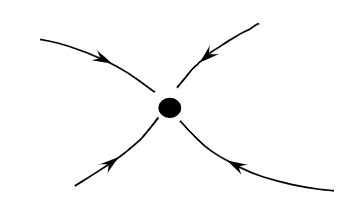
\includegraphics[width=4cm]{FixpunktAttraktor.png}
            & 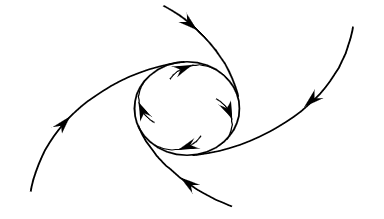
\includegraphics[width=4cm]{GrenzzyklusAttraktor.png}
            & 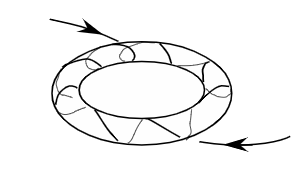
\includegraphics[width=4cm]{TorusAttraktor.png}
        \end{tabular}
        \captionof{figure}{Fixpunkt, Grenzzyklus, Tours- bzw. Ringattraktor \citep{Lueck}}
        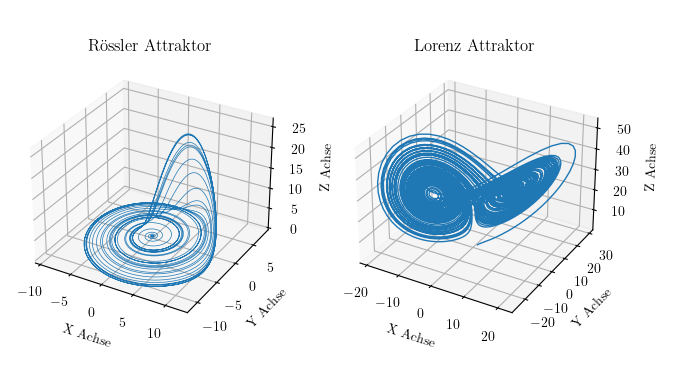
\includegraphics[width=14cm]{SeltsameAttraktoren.png}
        \captionof{figure}{Seltsame Attraktoren: Rössler- und Lorentzattraktor, Eigens erstellt mit dem Python Packages matplotlib mit Hilfe von \citep{py1, py2}}
    \end{center}
\end{itemize}

\subsection{Deterministisches Chaos}
\label{sub:determChaos}
Systeme, die das Verhalten des \textit{deterministischen Chaos} zeigen, weisen ein zufällig erscheinendes Verhalten auf, was jedoch nicht durch äußere Umstände verursacht wird, sondern das Verhalten folgt aus den Eigenschaften des Systems selbst.\\
Das Verhalten von einem System mit deterministischem Chaos lässt sich langfristig nicht vorhersagen, da ähnliche Uhrsachen langfristig nicht zu ähnlichen Wirkungen führen. Dieser Effekt ist unter dem Namen \textit{Schmetterlingseffekt} bekannt \citep{WikiDetChaos}.

\subsection{Fouriertransformation und Leistungsspektrum}
\label{sub:fouriertrafo}
Eine Fouriertransformation ist eine Integraltransformation, mit der aperiodische Signale in ein kontinuierliches Spektrum zerlegt werden können.\\
Fouriertransformation einer Messgröße \(x(t)\):
\begin{gather}
    \hat{x}(\omega) = \lim_{T \to \infty} \int_{0}^{T}  x(t) e^{-i\omega t}\,dt 
\end{gather}
Das Leistungsspektrum \( P(\omega)\) kann man nun folgendermaßen aus der Fouriertransformierten des Messwertes berechnen:
\begin{gather}
    P(\omega) = |\hat{x}(\omega)|^2
\end{gather}
Das Leistungsspektrum stellt die Leistungsanteile für unterschiedliche Frequenzen im Zeitsignal dar.\\
Bei chaotischen Systemen beispielsweiße erhält man ein Leistungsspektrum mit kontinuierlichem Verlauf, das für große Frequenzen abnimmt \citep{Lueck}. Da jedoch weißes stochastisches Rauschen ebenfalls ein kontinuierlichen Verlauf liefert kann dieser nicht als hinreichender Beweis für Chaos angesehen werden.

\subsection{Darstellungsweisen eines chaotischen Attraktor}
\label{sub:darstellungAttraktor}
\begin{itemize}
    \item[\textbf{1.}]{\textbf{Phasenraumdarstellung}}\\
    Die \textit{\textbf{Phasenraumdarstellung}} wie in (\ref{sec:allgemeines}) erwähnt, gibt einen Überblick über den Verlauf der Bewegung des dynamischen Systems. Dabei trägt man je an eine Raumachse eine Phasenraumvariabel auf (z.B. $x, \dot{x}$), wobei der Phasenraum dabei $n$-Dimensionen haben kann und nicht alle Phasenraumvariablen bekannt sein müssen, da ein Attraktor im Phasenraum rekonstruiert werden kann. Dazu werden die Messwerte einer Phasenraumvariablen bei einer festen Zeitspanne $\tau$, also $\varphi(t), \varphi(t+\tau)$,..., $\varphi(t+(n-1)\tau)$, als neu Koordinaten $x_i$ (z.B. $x_1=\varphi(t)~\text{und}~x_2=\varphi(t+\tau))$ eines neuen Koordinatensystems. Bei richtiger Wahl von $\tau$ und $n$ lässt sich dann der tatsächliche Attraktor rekonstruieren. Diese Methode der Rekonstruktion eines Atrraktors wurde vom Mathematik \textit{Floris Takens} bewiesen und ist auch als \textit{Einbettungstheorem} bekannt \citep{Lueck}.
    \item[\textbf{2.}]{\textbf{Poincar\'e-Abbildung}}\\
    Die \textit{\textbf{Poincar\'e-Abbildung}} ist eine Projektion des \textit{\textbf{Poincar\'e-Schnitts}} an einer Ebene. Diese Abbildung ist immer die Dimension $n-1$ und ist somit eine Dimension niedriger als der Phasenraum mit der Dimension $n$ und es gehen keinen Informationen bzgl. dem Langzeitverhalten des Systems verloren. Aufgrund dieser Tatsache lässt sich die \textit{Poincar\'e-Abbildung} zur Analyse von höherdimensionalen Phasenräumen verwenden.\\
    Der \textit{Poincar\'e-Schnitt} ist dabei eine Menge aller Durchstoßpunkte der Trajektorien im Phasenraum auf einer Hyperfläche. Hierbei müssen die Trajektorien die Hyperfläche \textit{transversal} (senkrecht) und in einer vorgegebenen Richtung schneiden. Praktisch werden meistens die Lage von Extremwerten einer Messgröße als Bedingung für die Schnittebene (Hyperfläche) und trägt diese gegen die anderen Phasenraumvariablen zu diesem Zeitpunkt gegeneinander auf oder man wählt eine Ebene, die den Attraktor geeignet schneide \citep{Lueck}.
    \item[\textbf{3.}]{\textbf{Wiederkehr-Abbildung}}\\
    Bei der \textit{\textbf{Wiederkehr-Abbildung}} wird eine diskrete Abbildung aktueller Messwerte über die vorangegangenen Messwerte aufgetragen. Dabei werden Punkte in einer $x(n)$-$x(n+1)$-Ebene aufgetragen mit den Messwerten $x_n$ als Koordinaten, also ($x_0,x_1$), ($x_1,x_2$),...,($x_n,x_{n+1}$). Diese Abbildung ähnelt dann einem \textit{Poincar\'e-Schnitt}, weswegen man bei einem kontinuierlichen System (\ref{eq:dynamDGL}) dessen \textit{Poincar\'e-Abbildung} für dieses Verfahren verwendet \citep{Lueck}.
    % TODO: #37 Recherche + Quelle zu Wiederkehrabbildung @ManeLippert
    \item[\textbf{4.}]{\textbf{Bifurkationsdiagramm}}\\
    Bei einem \textit{\textbf{Bifurkationsdiagramm}} betrachtet man die Projektion der \textit{Poincar\'e-Abbildung} auf \textbf{eine} Achse unter Veränderung eines Kontrollparameters, Parameter welche man aktiv im Experiment verändern kann, wobei man die durch die Projektion gewonnenen Werte gegen den jeweiligen Parameterwert aufträgt \citep{Lueck}.
    \item[\textbf{5.}]{\textbf{Phasendiagramm}}\\
    Wenn bei dem \textit{Bifurkationsdiagramm} mehrere unterschiedliche voneinander unabhängige Parameter existieren, verwendet man das \textit{\textbf{Phasendiagramm}}. Dazu trägt man die als Koordinatenachsen die jeweiligen Parameter, die das Systemverhalten beeinflussen, gegeneinander auf und erhält Landkarte des globalen Systemverhaltens in Abhängigkeit der gewählten Parameter \citep{Lueck}.  
\end{itemize}
% Manuel Lippert - Paul Schwanitz
% Physikalisches Praktikum

% Teilaufgabe 2

\section{Das invertierte Pendel}
\label{sec:invertPendel}
Das invertierte Pendel erzeugt eine \textit{nichtlinearer} Schwingung. Dabei besitzt das Pendel eine unten fest eingespannte Blattfeder mit Federkonstante $k$, welche über zwei horizontal in der Höhe $h$ und der Auslenkung $x_h$ angreifende Spiralfedern mit Federkonstante $k_s$ und der Auslenkung $\hat{x}$ angetrieben wird. Am oberen Ende der Blattfeder lässt sich ein Zusatzgewicht $M$ anbringen und der Winkel $\theta$ beschreibt den Winkel zwischen der Tangenten an der Pendelspitze und dem Lot. Weiterhin bezeichnet die Pendellänge $L$ die Länge zwischen dem Anfang und Ende der Blattfeder, welche vom Winkel $\theta$ abhängt (siehe Abb \ref{image:invertiertesPendel}).
\begin{center}
    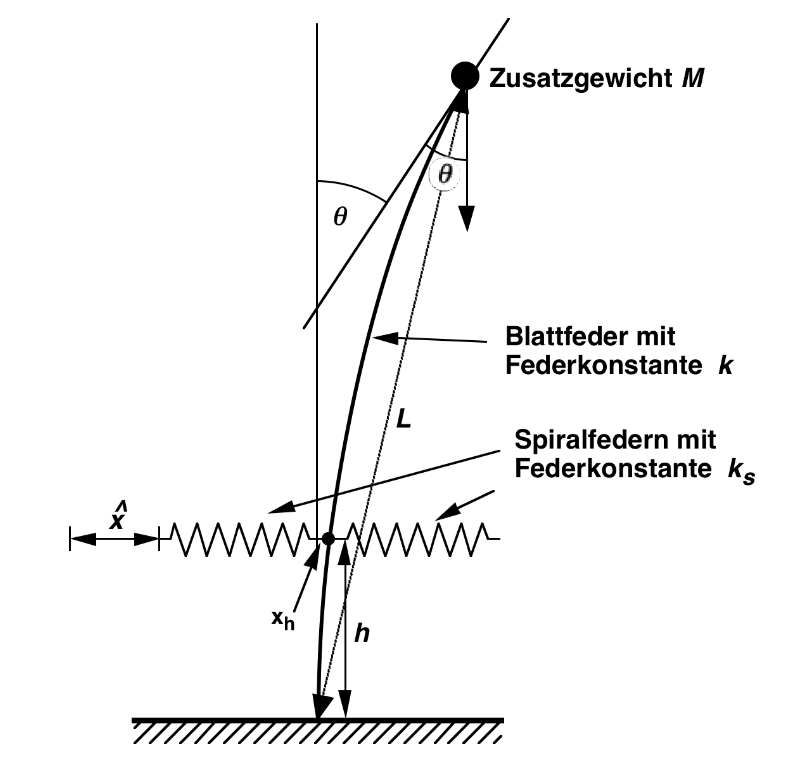
\includegraphics[scale=0.25]{Pendel/invertiertesPendel.png}
    \captionof{figure}{Skizze invertiertes Pendel \citep{Lueck}}
    \label{image:invertiertesPendel}
\end{center}
\subsection{Herleitung der Bewegungsgleichung}
\label{sub:bewegungsgleichung}
Die Bewegungsgleichung lässt sich über die wirkenden Drehmomente der Bauteile bestimmen:
\begin{gather*}
        \text{Pendel}~+~\text{Dämpfung}~+~\text{Blattfeder}~-~\text{Spiralfedern}~-~\text{Gewicht} = 0
\end{gather*}
\begin{gather}
    \Rightarrow [M(L(\theta))^2\ddot{\theta}]+[2\delta\dot{\theta}]+[k\theta]-[hk_s(x_h+\hat{x}\cos(\omega t))]-[MgL(\theta)\sin(\theta)]=0
\end{gather}
Dabei bezeichnet $\delta$ die Dämpfungskonstante und $g$ die Erdbeschleunigung.\\
Im Folgenden wird die Pendellänge $L$ als konstant angenommen, obwohl diese nicht konstant ist und von der Art der verwendeten Masse $M$ abhängt. Weiterhin wird die Auslenkung $x_h$ als vernachlässigbar klein angesehen und der Angriffswinkel der Spiralfedern wird als $\frac{\pi}{2}$ genähert, was bei genügend kleiner Höhe $h$ gegeben ist.
Daraus folgt die genäherte Form der Bewegungsgleichung:
\begin{gather}
    ML^2\ddot{\theta}+2\delta\dot{\theta}+k\theta-MgL(\theta)\sin(\theta)=hk_s\hat{x}\cos(\omega t)=T_0\cos(\omega t)
\end{gather}
Wobei $T_0$ als die Amplitude des periodisch angreifenden Drehmoments interpretiert werden muss. Hierbei ist noch zu erwähnen, dass durch die Näherungen die Lösung dieser Differentialgleichung nicht der tatsächlichen Trajektorien des Systems entsprechen, da diese stark von der Anfangsbedingung abhängen, dennoch ist eine globale Aussage über das Verhalten mit der genähreten Differentialgleichung möglich.\\
Zu den letzten beiden Termen lässt sich dann ein Potenzial definieren und durch Entwicklung des Cosinus für kleine Winkel $\theta$ (Kleinwinkelnäherung KWN) bis zur 2.Ordnung ergibt sich das Potenzial des \textit{Duffing-Oszillator} \citep{Lueck}.
\begin{gather}
    V(\theta) = \frac{1}{2}k\theta^2 + MgL(\cos(\theta)-1)\overset{\text{KWN}}{\approx}\frac{1}{2}(k-MgL)\theta^2 + \frac{1}{24}MgL\theta^4~,V(0)=0
\end{gather}

\subsection{Symmetriebrechung}
\label{sub:symbrechung}
Bei einer {kritischen Masse} $M_k=\frac{k}{gL}$ erfährt das System des Pendels einen Übergang von einem monostabilen System ($M<M_k$) in ein bistabiles System ($M>M_k$), dabei ist die Bewegung des Pendels in beiden Fällen Unterschiedlich und muss deshalb getrennt betrachtet werden. Bei diesem Übergang verändert sich die Struktur des Potenzial (siehe Abb \ref{image:potPendel}), wodurch nun zwei Lösungen für das System möglich sind. Das Auftreten von mehreren Lösungen in einem System wird dann auch \textit{\textbf{Symmetriebrechung}} genannt \citep{Lueck}.
\begin{center}
    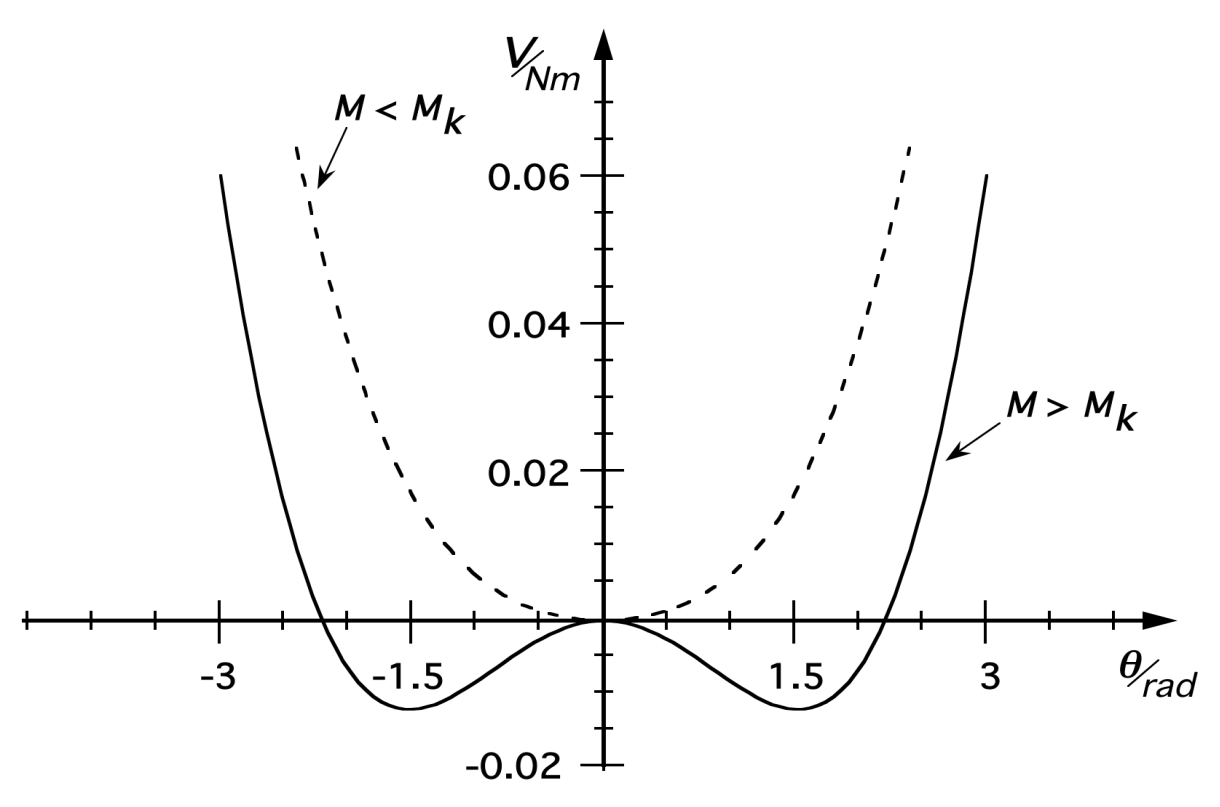
\includegraphics[scale = 0.2]{Pendel/PendelPotenzial.png}
    \captionof{figure}{Potenzialdarstellung für invertiertes Pendel \citep{Lueck}}
    \label{image:potPendel}
\end{center}

\subsection{Schwingungsdauer in Abhängigkeit der Masse}
\label{sub:schwingungsdauer}
Bei einem nichtlinearen Pendel hängt, im Gegensatz zu einem linearen Schwingungsvorgang, die Resonanzfrequenz $\omega_r$ von der Schwingungsamplitude $b$ ab $\Rightarrow \omega_r(b)$. Unverändert bleibt dennoch die Schwingungsamplitude $b(\omega)$ gegenüber der Resonanzkurve eines linearen Oszillators bei unterschiedlichen Anregungsfrequenzen $\omega$ \citep{Lueck}.
\begin{itemize}
    \item[1.] $M<M_k$ (Schwache Nichtlinearität)\\
    Pendel ist nach (\ref{sub:symbrechung}) monostabil. Der Vorgang lässt sich näherungsweise mit der Bewegungsgleichung eines Duffing-Oszillator nähern, wobei die Abhängigkeit der Resonanzfrequenz $\omega_r$ von der Amplitude $b$ berücksichtigt bleibt. Die Bewegungsgleichung lautet in diesem Fall:
    \begin{gather}
        \ddot{\theta} + 2\delta\dot{\theta} + \omega_0^2\theta + \gamma\theta^3 = f_a\cos(\omega t)
    \end{gather}
    Dabei bezeichnet $\gamma$ den Faktor der Nichtlinearität, $\omega_0$ die Resonanzfrequenz des Systems ohne Nichtlinearität ($\gamma=0$), $f_a$ die Anregungsamplitude mit Anregungsfrequenz $\omega$ und $\delta$ die Dämpfung.\\
    Durch Betrachtung des Verlaufs der Resonanzkurve in der Nähe von $\omega_0$ erhält man eine Gleichung dritter Ordnung für das Quadrat der Schwingungsamplitude $b$.
    \begin{gather}
        \left[\left((\omega^2-\omega_0^2) - \frac{3}{4}\gamma b^2\right)^2+(2\delta\omega)^2\right]b^2=f_a^2 %Angepasst an die Form in Wikipedia https://en.wikipedia.org/w/index.php?title=Duffing_equation&oldid=1031816809
        \label{eq:resonanzkurve}
    \end{gather}
    Diese Gleichung hat je nach Werten von $f_a, \gamma, \omega_0~\text{und}~\delta$ eine reelle oder zwei konjugierte komplexe Lösungen.
    Dabei ist es einfacher die Gleichung nach $\omega$ aufzulösen, wobei zur Vereinfachung $\omega_0=1$ angenommen wird. Damit wird (\ref{eq:resonanzkurve}) zu:
    \begin{gather}
        \left[\left((\omega^2-1) - \frac{3}{4}\gamma b^2\right)^2+(2\delta\omega)^2\right]b^2=f_a^2
    \end{gather}
    Mit der Lösung für $\omega$:
    \begin{gather}
        \omega^2_{1,2} = 1 - 2\delta^2 + \frac{3}{4}\gamma b^2 \pm \sqrt{\frac{f_a^2}{b^2}+ 4\delta^2\left[\delta^2 - \left(1 + \frac{3}{4}\gamma b^2\right)\right]}
    \end{gather}
    Bei hinreichender kleinen Dämpfung $\delta$ gibt es zwei verschiedene eingeschwungene Zustände, da die Lösung instabil wird (siehe Abb \ref{image:resonanzkurve}c)).
    \begin{center}
        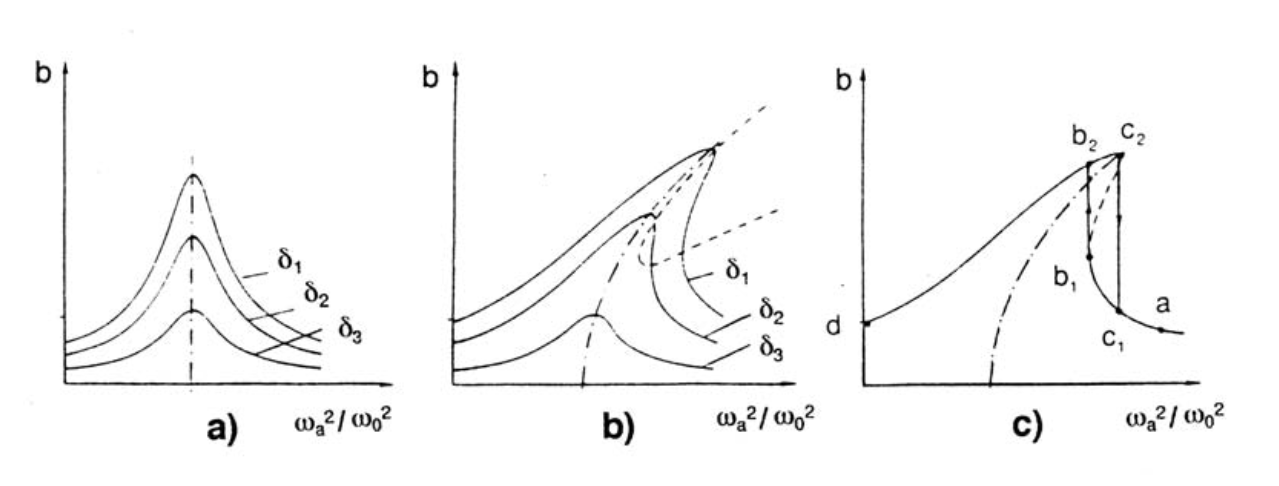
\includegraphics[scale=0.3]{Pendel/Resonanzkurve.png}
        \captionof{figure}{Resonanzkurven für eines Duffing-Oszillator \citep{Lueck}}
        \label{image:resonanzkurve}
        \captionof*{figure}{a) linearer ($\gamma=0$) b) nichtlinear c) Hysterese}
    \end{center}
    % https://www.ila.uni-stuttgart.de/nlvib/downloads/HB_NLvib_presentation.pdf, https://www.hindawi.com/journals/mpe/2011/248328/
    Die Schwingungsdauer $T$ hängt hierbei logarithmisch von der Amplitude $b$ ab mit dem Zusammenhang:
    \begin{gather}
        T = T_0 + T_1\log(b)
    \end{gather}
    Dies geht aus experimentellen Daten von \citep{Lueck} hervor, wobei $T_0$ und $T_1$ Näherungsparameter sind.
    \item[2.] $M>M_k$ (Starke Nichtlinearität)\\
    Das Pendel ist in diesem Fall nach (\ref{sub:symbrechung}) bistabil und besitzt zwei stabile Ruhelagen. Durch die Verringerung von großen Antriebsfrequenzen $\omega$ entstehen nach Ende des Einschwingverhaltens nacheinander subharmonische Schwingungen mit einer Periodenverdopplungskaskade ($T_n=2^nT=2^n\frac{2\pi}{\omega}$), obwohl sich das Pendel unterhalb einer kritischen Frequenz $\omega_k$ chaotisch verhält. Dieses Verhalten ist auch ein Beispiel für ein Bifurkationsszenario \citep{Lueck}.
\end{itemize}
\newpage
\subsection{Aufbau Pendel}
\label{sub:aufbauPendel}
\begin{center}
    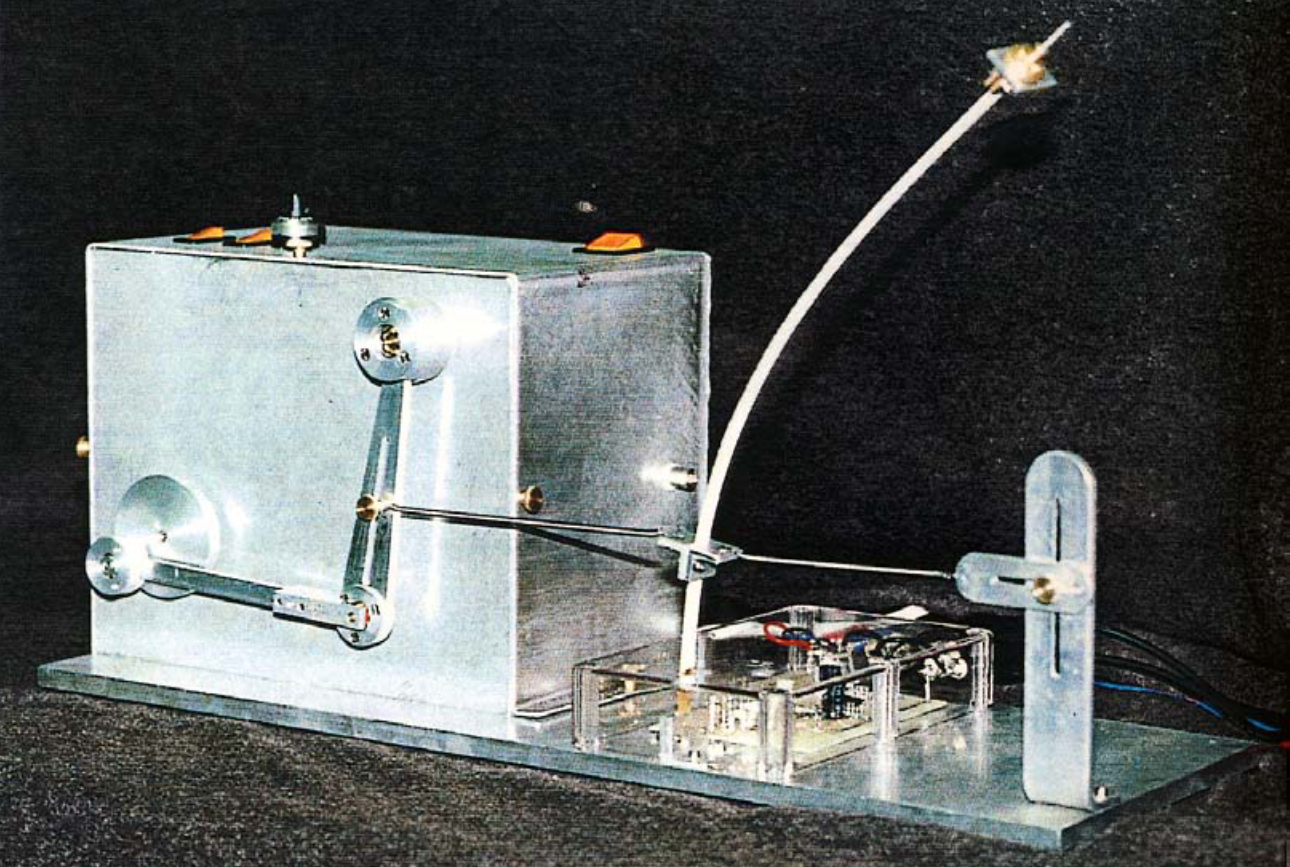
\includegraphics[scale=0.25]{Pendel/AufbauPendel.png}
    \captionof{figure}{Aufbau des invertierten Pendels \citep{Lueck}}
    \label{image:aufbauPendel}
\end{center}
Hierbei besteht das Pendel aus einer:
\begin{itemize}
    \item 5 mm starken Aluminium-Grundplatte
    \item 1 cm x 15 cm x 40 cm lange Blechstreifen aus einer Messing-Legierung mit hohem Kupferanteil, Dehnungsmessstreifen auf beiden Seiten (DMS, Widerstand abh. von der Dehnung) knapp oberhalb der Befestigung $\rightarrow$ Blattfeder
    \item Spiralfedern mit Federkonstante $k=027$ N/cm 
    \item Schrittmotor im Gehäuse mit 200 bzw. 400 Schritten (Halbschrittbereich)
    \item Multifunktionskarte Typs DAS 1602 der Firma Keithley (Taktimpulsgeber für Schrittmotoren)
\end{itemize}
Mit diesem Aufbau sind bis zu ca 5 Umdrehungen/s möglich, wobei die Antriebskraft durch das Verändern des Angriffspunktes der Spiralfeder am Übertragungshebel variierbar ist \citep{Lueck}.

\subsection*{Funktionsweise Differenzier-Schaltung}
Bei einer Differenzier-Schaltung wird nur die Änderung der Eingangsspannung zu einer Ausgangsspannung verarbeitet. Dabei wird ein Kondensator am Eingang in Reihe und ein Widerstand parallel zwischen Eingang und Ausgang des Operationsverstärker geschaltet. Durch den Kondensator fließt nur Strom, wenn sich die Eingangsspannung ändert, wobei die Ausgangsspannung proportional zur Änderungsgeschwindigkeit der Eingangsspannung ist. Durch den Operationsverstärker wird dann das Signal verstärkt, um dieses Signal besser über ein angeschlossenes Messgerät (z.B. Oszilloskop) betrachten zu können \citep{electronik}.

\begin{center}
    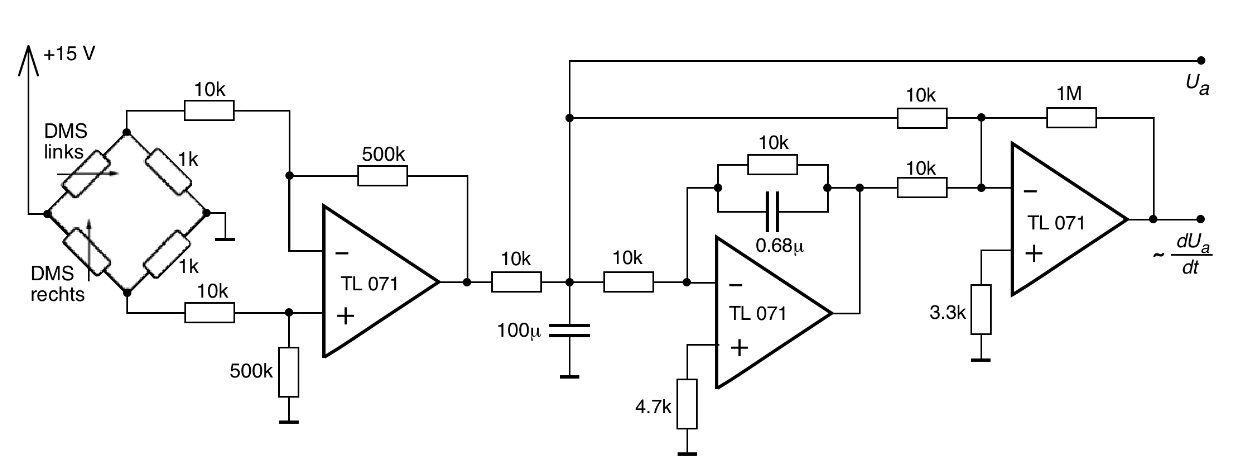
\includegraphics[scale=0.3]{Pendel/MessschaltungPendel.png}
    \captionof{figure}{Messschaltung des invertierten Pendels \citep{Lueck}}
    \label{image:schaltungPendel}
\end{center}
Für die Messschaltung (siehe Abb. \ref{image:schaltungPendel}) wird für eine höhere Genauigkeit zwei DMS in einer Brückenschaltung verschalten, um die Spannungsdifferenz von ihnen zu messen, wobei die Spannung dann proportional zur Pendelauslenkung $\theta$ ist. Für das Abgreifen der Geschwindigkeit als zweite Phasenraumvariable werden die Spannungen über eine Operationsverstärker-Schaltung differenziert. Die Spannungen werden dann einem im PC eingebauten Analog-Digital-Wandler-Karte gemessen, wobei die Messkarte über LABVIEW (Messprogramm) gesteuert wird \citep{Lueck}.
% Manuel Lippert - Paul Schwanitz
% Physikalisches Praktikum

% Teilaufgabe 3
\newpage
\section{Der Shinriki-Oszillator}
\label{sec:shinrikiOszi}


\subsection{Differentialgleichung und Aufbau des Shinriki-Oszillator}
\label{sub:dgl}

\begin{figure}[h]
    \centering
    %TODO #31
    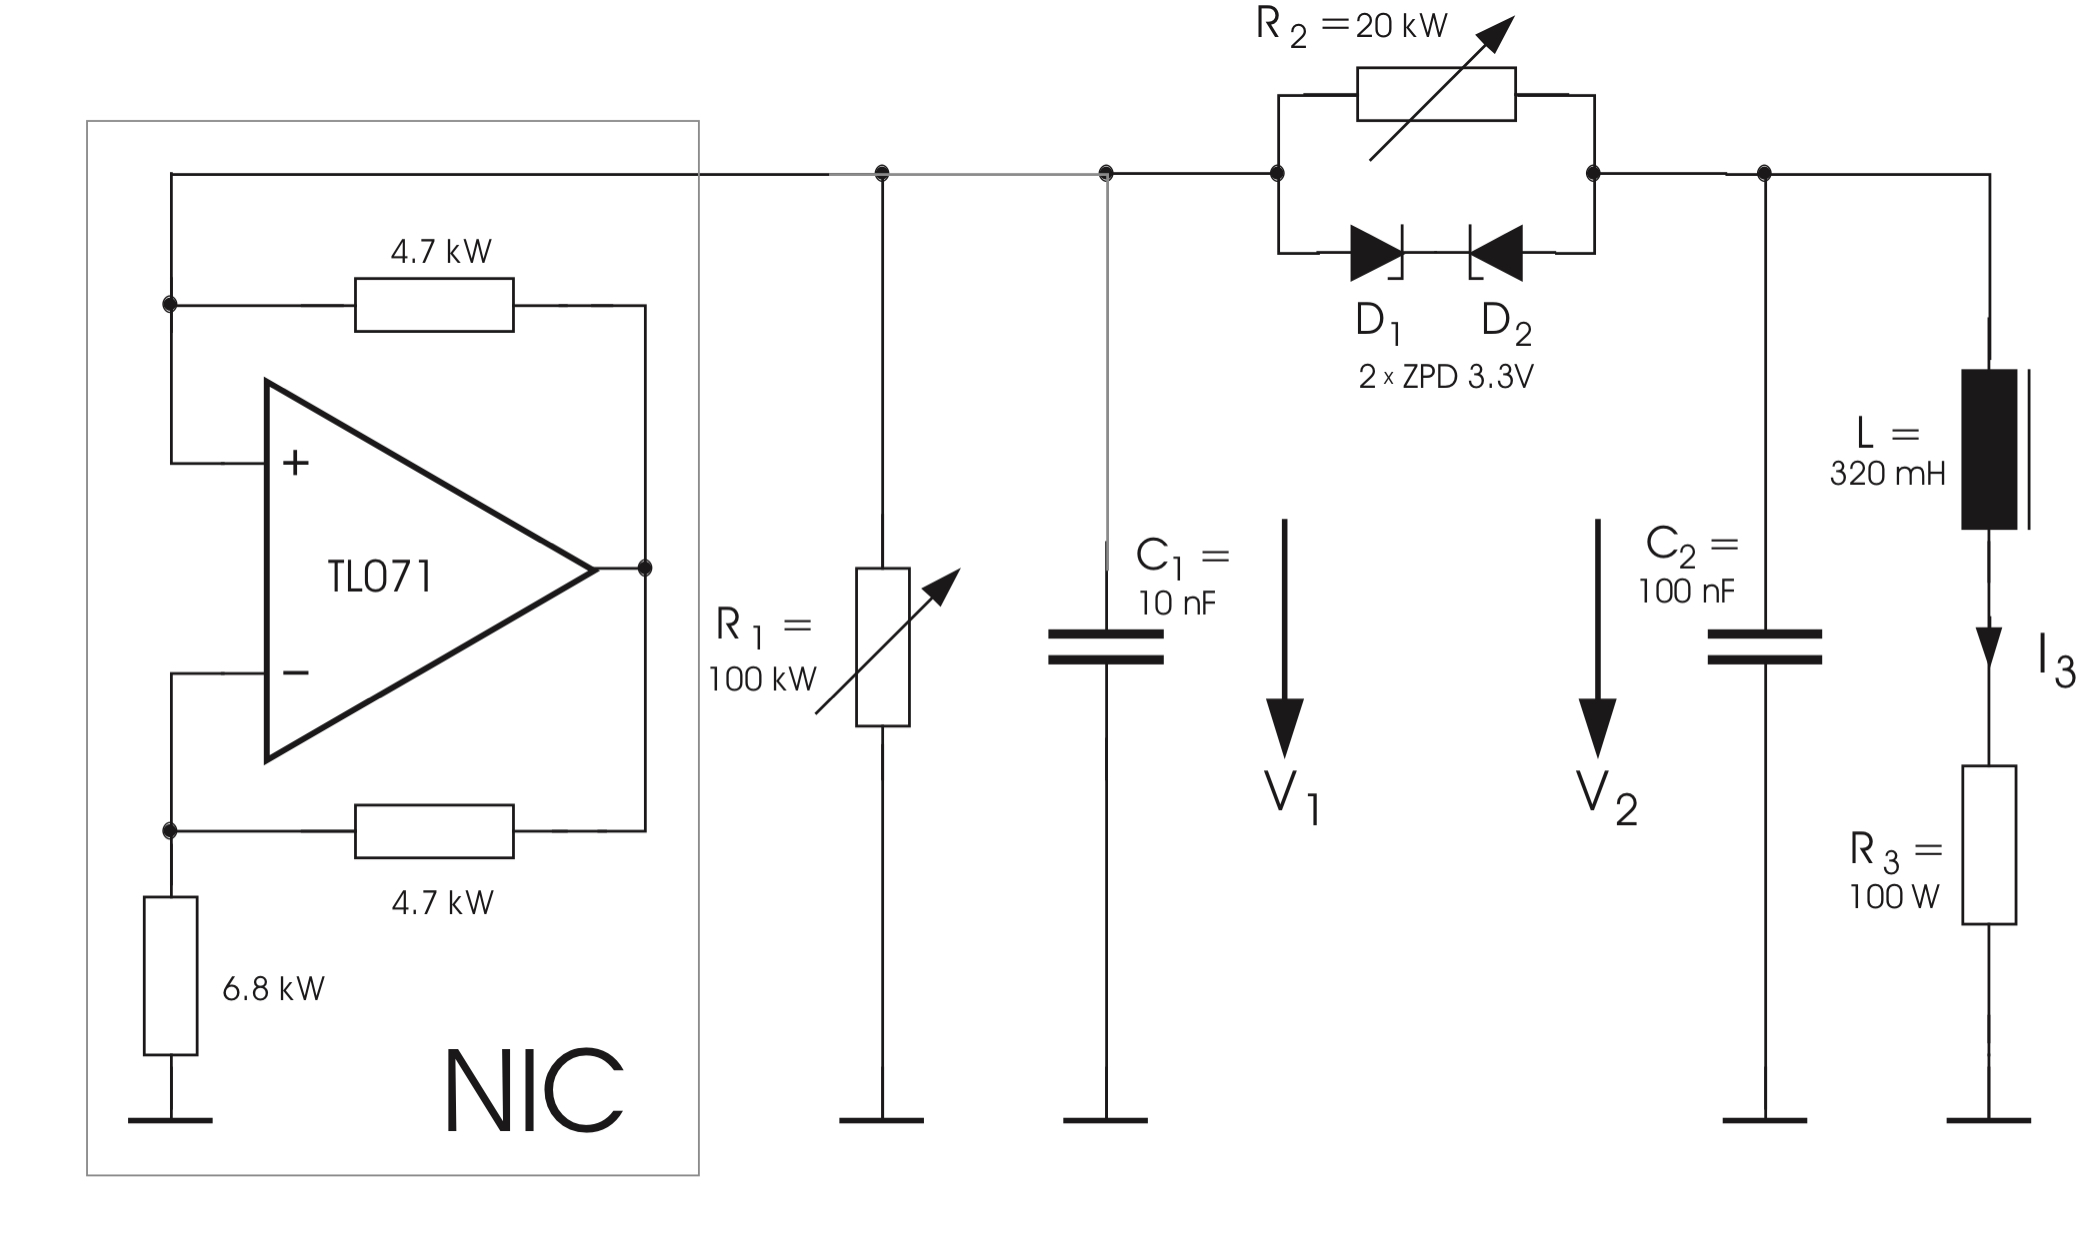
\includegraphics[scale=0.15]{ShinrOsziSp.jpeg}
    \label{fig:shinrikiSp}
    \caption{Schaltplan des Shinriki-Oszilator \citep{Lueck}}
\end{figure}

Der Shinriki-Oszillator besteht aus einem negativen Impedanzkonverter (NIC) und einem LC-Parallelschwinkreis, die durch ein gegeneinader geschaltetes Zenerdiodenpaar und dem parallel geschalteten \(R_2\), gekoppelt sind. \\
Die Leitwertfunktion des Kopplungsglied ist \( f(V)\) und beschreibt den Strom, der über das Kopplungsglied fließt.
\(R_{NIC}\) ist der Widerstand des NIC innerhalb des relevanten Intervalls von -8,1 V bis 8,1 V \citep[]{Lueck}.\\
Damit und mit den Kirchhoffschen Regeln lassen sich nun die DGLs aufstellen:
\begin{align}
    C_1 \dot{V_1} &= V_1 (\frac{1}{R_{NIC}}-\frac{1}{R_1}) - f(V_1-V_2) \\
    C_2 \dot{V_2} &= f(V_1-V_2) - I_3 \\
    L \dot{I_3} &= -I_3R_3 + V_2
\end{align}

\subsection{NIC und Schwingung des Shinriki-Schaltkreis}
\label{sub:nic}
Ein NIC benutzt einen Operationsverstärker, um einen negativen ohmschen Wiederstand zu simulieren. Hierbei wird der gewünschte Widerstand einfach zwischen dem (-) Eingang des OpAmp und GND geschaltet. Durch den OpAmp wird ein Widerstand mit negativem Wert des eben eingesetzten simuliert. \\
Daher mus das System nicht mehr von außen zur Schwingung angeregt werden.
% TODO #29

\subsection{Geräusche einer Bifurkation}
\label{sub:tonBifurkation}
Eine Bifurkation ist eine verdopplung der Periodendauer, d.h. die Frequenz wird halbiert. Dies verursacht einen tieferen Ton.
% TODO #30

% etc.

    % 3.Kapitel Protokoll
    % Charlotte Geiger - Manuel Lippert - Leonard Schatt
% Physikalisches Praktikum

% 3.Kapitel  Protokoll

% Variables
\def\skalierung{0.65}

\chapter{Messprotokoll}
\label{chap:protokoll}

Das Messprotokoll wurde am Versuchstag handschriftlich erstellt und hier als
PDF-Datei eingefügt. 

\section*{Zusatz}
Zusätzlich fügen wir die Bilder und die verwendeten Schaltungen des Versuchs nch dem Protokoll an zur besseren Übersicht.

% Einbindung des Protokolls als pdf (mit Seitenzahl etc.)
% Erste Seite mit Überschrift
%\includepdf[pages = 1, landscape = false, nup = 1x1, scale = \skalierung , pagecommand={\thispagestyle{empty}\chapter{Protokoll}}]
%            {03-Protokoll/Protokoll.pdf}
% Restliche Seiten richtig skaliert
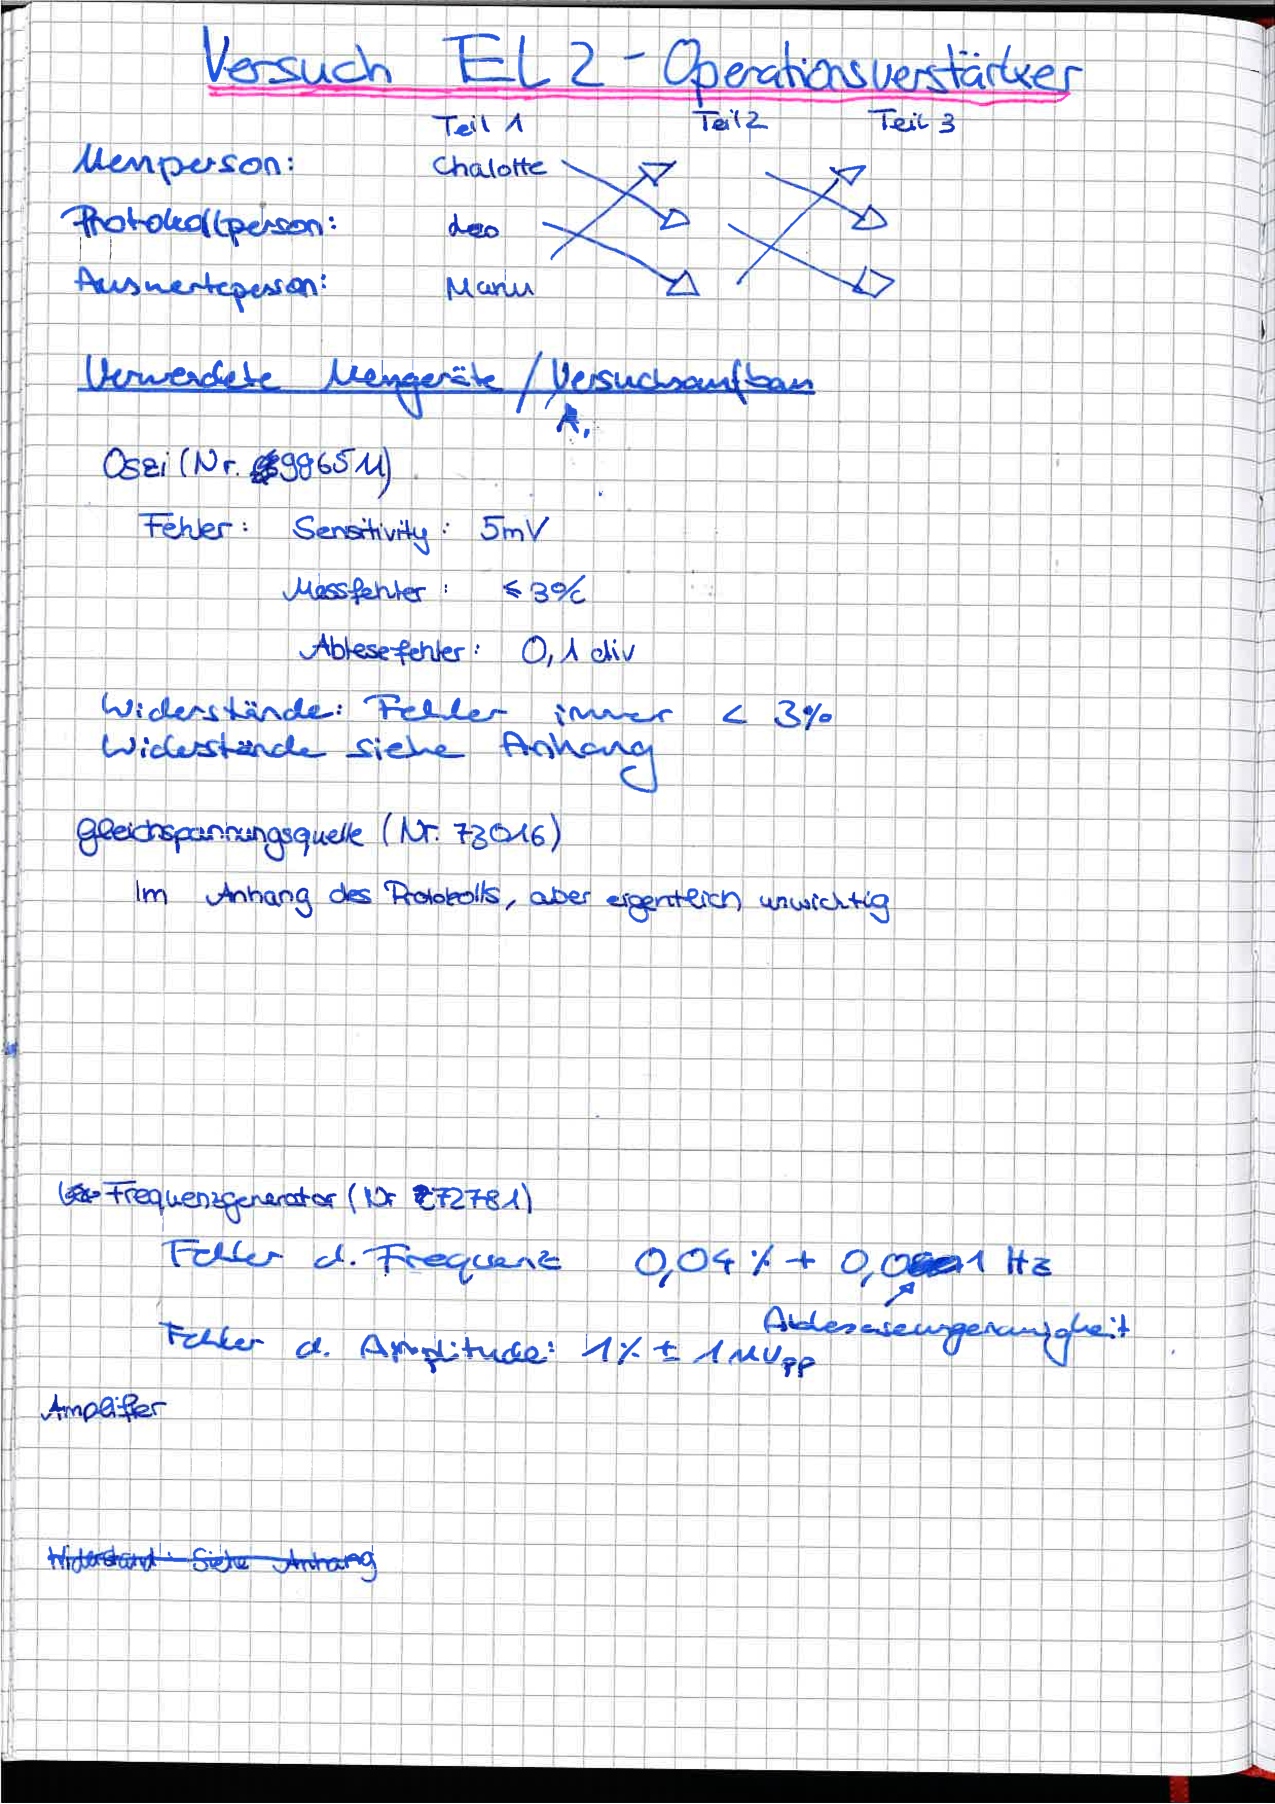
\includepdf[pages = -, landscape = false, nup = 1x1, scale = \skalierung , pagecommand={}]{30-ProtokollEL2.pdf}

%\section*{Steckbretter}
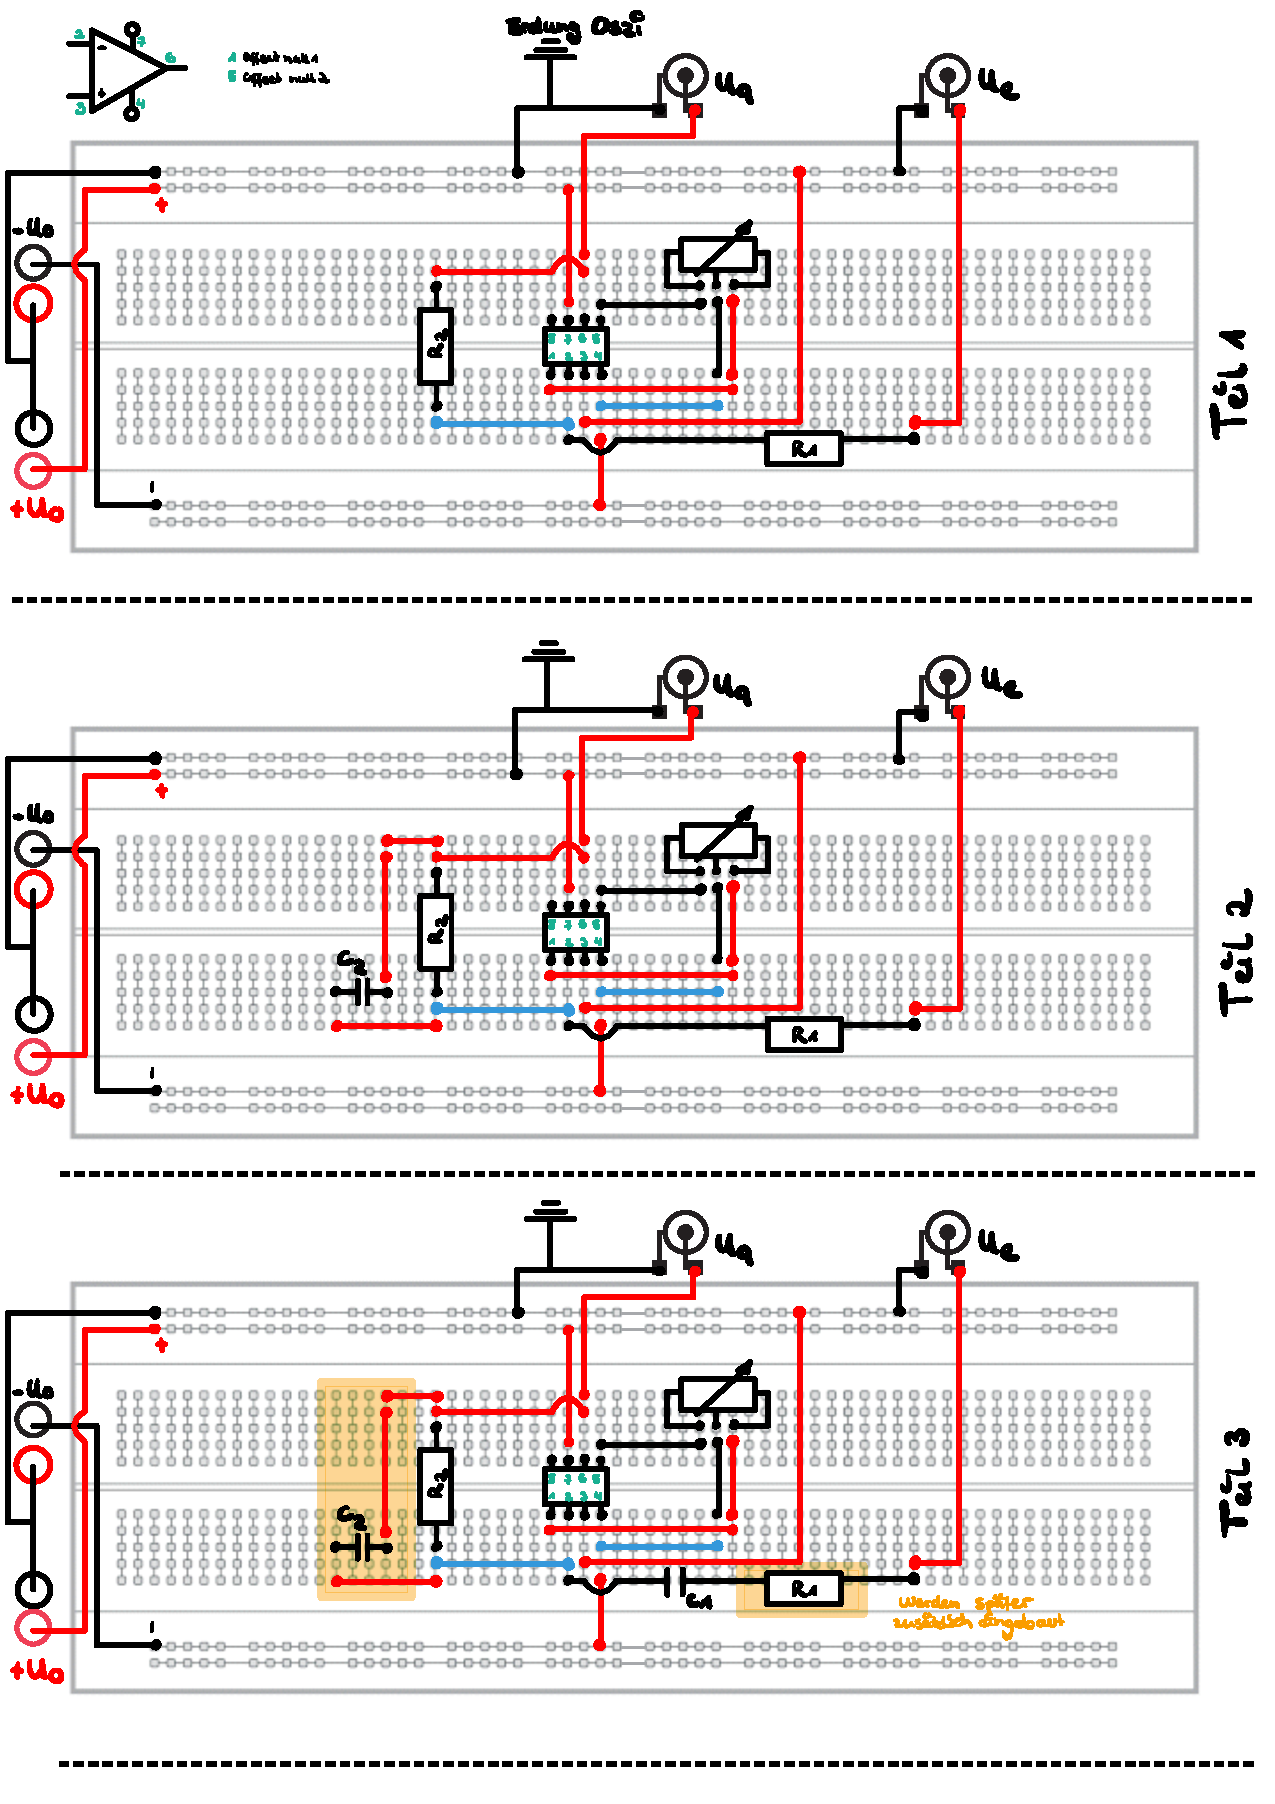
\includepdf[pages = 1, landscape = false, nup = 1x1, scale = \skalierung , pagecommand={}]{30-SteckbretterEL2.pdf}


    % 4.Kapitel Versuchsauswertung
    % Manuel Lippert - Paul Schwanitz
% Physikalisches Praktikum

% 4.Kapitel Versuchsauswertung

\chapter{Auswertung und Diskussion}
\label{chap:versuchsauswertung}

% Text

% Input der Teilauswertung je nach Produktion der Nebendateien ohne Ordner
%Matteo Kumar - Leonhard Schatt
% Fortgeschrittenes Physikalisches Praktikum

% Teilauswertung X

\section{Teilauswertung X}

% etc.

    % 5.Kapitel Fazit
    % 5. Fazit

\chapter{Fazit}
\label{chap:fazit}


% Text

    % Anhang
    %% Matteo Kumar - Leonard Schatt
% Physikalisches Praktikum

% Anhang

\appendix

% Text

% Charlotte Geiger - Manuel Lippert - Leonard Schatt
% Physikalisches Praktikum

% Anhang A

\chapter{Append A}
\label{chap:anhangA}

\section{Teilanhang X}


    % Literatur

    % TODO: #26 Abbildungsverzeichnis @ManeLippert@PaulSchwanitz
    \bibliographystyle{Auswertung.bst}
    \nocite{*}
    \bibliography{Auswertung.bib}

    %Abbildungsverzeichnis
    \listoffigures
    % TODO: #36 Quellen der Abbildungen @ManeLippert

\end{document}